\vspace{5 mm}  %to enter vertical space
\subsection*{What is LibreCAD$?$}
LibreCAD is a free, open source 2D CAD software for Windows, Apple, Linux. It is released under the license of  GNU General Public License(GPL v2).
\subsection*{Why LibreCAD$?$}
It is a CAD software used to create 2D drawings. It has many fascinating features that would help you to add more details to your drawings. It is a perfect 2D CAD software and is light weighted. It is available for Windows, Apple, Linux.
\subsection*{I am new to LibreCAD, How could I start$?$}
If you are new to CAD, don't worry, this notes will help you to learn some CAD concepts too. This quick start notes will help you to start creating drawings in LibreCAD quickly.\\
\subsection*{Getting familiar with User Interface}
LibreCAD has an interactive user interface. One can easily get familiar with it.
\begin{figure}[h!]
\centering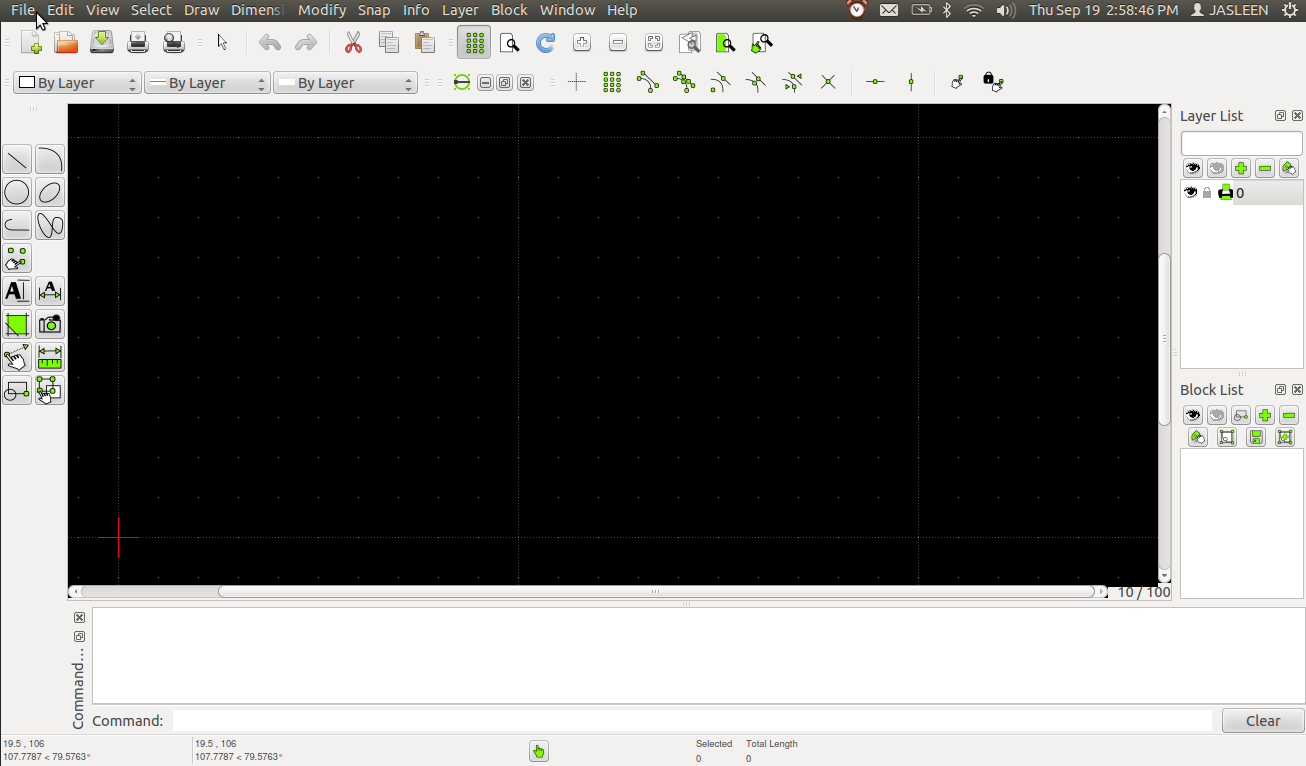
\includegraphics[width=450px]{./images/screen.png}
\caption{\small \sl User Interface of LibreCAD}
\end{figure}\\
%
\subsection*{LibreCAD window is divided into eight areas:}
\begin{enumerate}
\item{Menubar}
\item{Toolbar}
\item{Model Space}
\item{Layer Selection Box}
\item{Command Line}
\item{Status Line}
\item{Layer List}
\item{Block List}
\end{enumerate}
%
\begin{figure}[h!]
\centering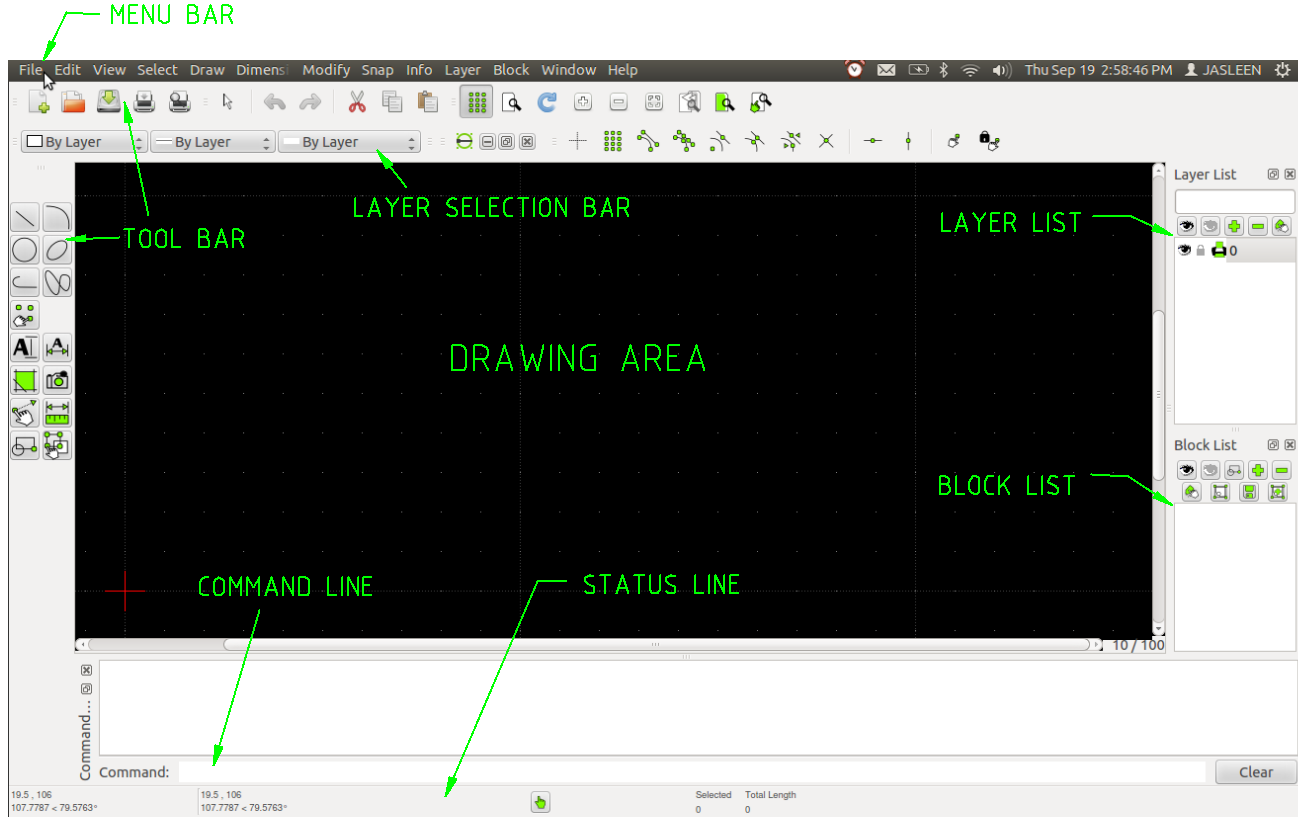
\includegraphics[width=450px]{./images/labelscreen.png}
\caption{\small \sl LibreCAD Screen}
\end{figure}
%
\textbf{\\\underline{Menu Bar:}}
A horizontal menu located on top that contains the major functions of CAD. When a function is selected from the menu, the menu drops down and displays further options under the menu. A number of options in the menu bar allows you to set program defaults and create a customized working environment.
\\\\
\textbf{\underline{Toolbar:}}
A collection of tool buttons grouped together. It is on the left side of the drawing window. Using tool bars is a very convenient method of entering commands, because you don't need to type on the keyboard or navigate through the menus. Each command is represented with a specific tool button in the tool bar. To enter a command, all you need to do is click on the tool button with the help of pointing device. It has nested toolbar in it. If you select circle, then it will display a varity of circles under a `circle' category. There is also a toolbar below the menu bar, which contains some common functions. LibreCAD allow you to customize the toolbars as needed. You can place
frequently used tool buttons in a tool bar, display only specific tool bars, and arrange them on the screen as you like.\\\\
\textbf{\underline{Model space/Drawing window:}}
The Drawing window or Model space is the area where you create your drawing. All the drawing work is confined within this area. The drawing
window may look small, but it has infinite size like the sky. You can draw as big or as small on this sky like drawing window. The view-display functions allow you to display specific views of the drawing.\\\\
\textbf{\underline{Layer Selection Box:}}
Layer Selection Box helps in selecting the Layer's atributes like: color, line type, thinkness.\\\\
\textbf{\underline{Command Line:}}
It is used to type commands. It notify you warnings or errors, if something is wrong. An area on the screen that shows all the commands being entered. You just need to remember the command names and type in command window to perform its function. Like, if you want to draw circle, then type `circle' in command window, it will ask you to enter the coordinates where to draw circle and with what radius.\\
Working with command window is fast and accurate method to draw. But you have to remember the command names to perform its function. These commands also has short commands, like to draw line, you can type 'line', 'ln' or 'l'\\\\
\textbf{\underline{Status Line:}}
The bottom bar of your screen which shows status of LibreCAD. Shows settings associated with the current drawing on the screen. It shows absolute and relative position of your mouse in cartesian and in polar coordinates. The mouse widgets shows the status of mouse left and right button. The `Selected Entities' shows you number of entities you selected. To enable/disable status bar, goto menu:  view $>$ status bar.\\\\
\textbf{\underline{Layer/ Block List:}}
It is on the right side of the drawing window. It shows the Layers and Blocks of currently opened Drawing.\\
\textbf{Layers} are used to keep same type of attributes in one layer. we can toggle the layers i.e to change the layers visible to hidden or vice-versa.\\
\textbf{Blocks} are used to use the block of a drawing, many times in our drawing.\\\\
%
\subsection*{\underline{Ways to communicate with LibreCAD:}}
\begin{itemize}
\item{Using the Menu Bar.}
\item{Using the tool bars.}
\item{Entering commands in the command window.}
\item{Working in the drawing area.}
\end{itemize}
%
\subsection*{\underline{Checking Version of LibreCAD:}}
It is important to check version of LibreCAD before starting work. LibreCAD version shoud be $>$=v2.0.*
If you have LibreCAD version less than this, then kindly switch to latest version as, the old version contains some bugs.
To check the version of your Application. Goto Help menu $>$ Select About. Ensure here the version of LibreCAD you using.\\\\
\begin{figure}[h!]
       \centering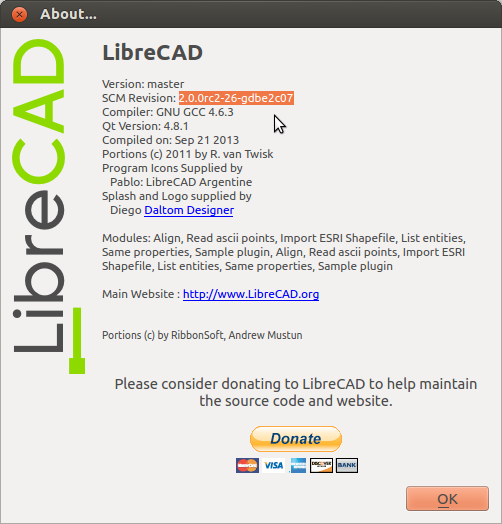
\includegraphics[width=230px]{./images/about.png}
       \caption{\small \sl About LibreCAD}
       \end{figure}
